\documentclass[12pt]{article}

\usepackage{times}
\usepackage{amsmath}
\usepackage{latexsym}
\usepackage{fullpage}
\usepackage{graphicx}
\usepackage{amsfonts}

\graphicspath{ {./images/} }

\newcommand{\NOT}{\neg}
\newcommand{\AND}{\wedge}
\newcommand{\OR}{\vee}
\newcommand{\XOR}{\oplus}
\newcommand{\IMPLIES}{\rightarrow}
\newcommand{\IFF}{\leftrightarrow}
\newcommand{\E}{\exists}
\newcommand{\A}{\forall}

\setlength{\parskip}{.1in}

\renewcommand{\baselinestretch}{1.1}

\begin{document}

\begin{center}

{\bf
CSCE 463\\
HW 2 Report\\
Jeffrey Xu\\
03/16/21\\
}

\end{center}

\section{Case 1}

\subsection{random0.irl}

We needed to test \emph{random0.irl} with the provided DNS server. The following output/trace of the program is shown below.

\begin{center}
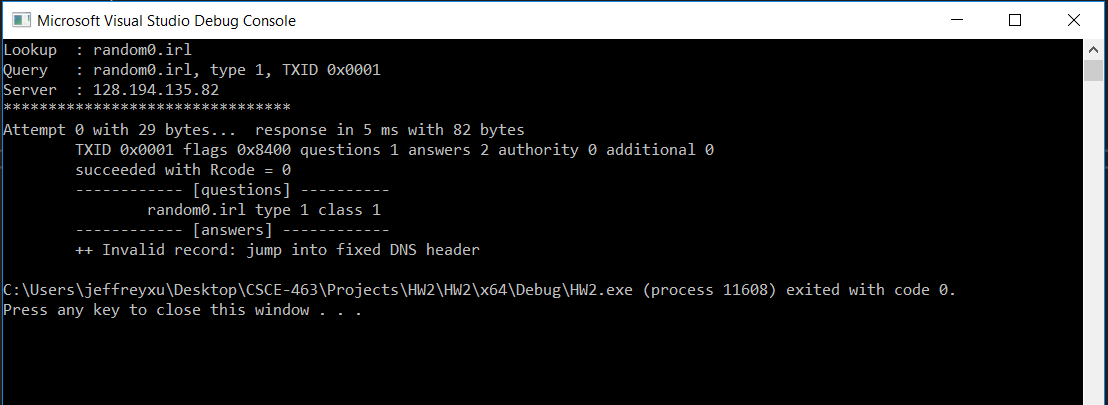
\includegraphics[width=11cm, height=4cm]{random0.irl}
\end{center}

We can see that there apppeared to be a jump into the fixed DNS header. The Wireshark output for the packet is shown below.

\begin{center}
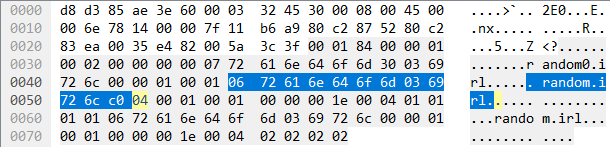
\includegraphics[width=11cm, height=3cm]{random0.irlWireShark}
\end{center}

We can clearly see that after the last \emph{random.irl}, there seems to be a jump but to an offset that is clearly within the fixed DNS header (4 is between 0 and 12 which is the fixed DNS header length). Therefore, the error output is valid. 

\subsection{random3.irl}

Now we want to test \emph{random3.irl} on the given server. The output is shown below.

\begin{center}
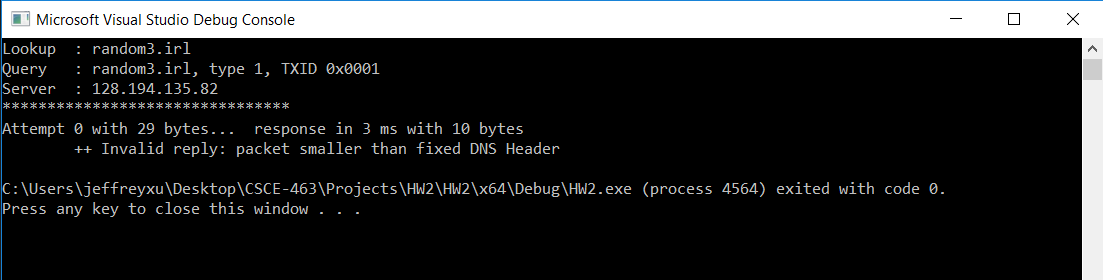
\includegraphics[width=11cm, height=3cm]{random3.irl}
\end{center}

We can clearly see that the response is only 10 bytes making it smaller than the fixed DNS header which is 12 bytes by default. To further prove that this response is incorrect, the Wireshark response is also shown below. 

\begin{center}
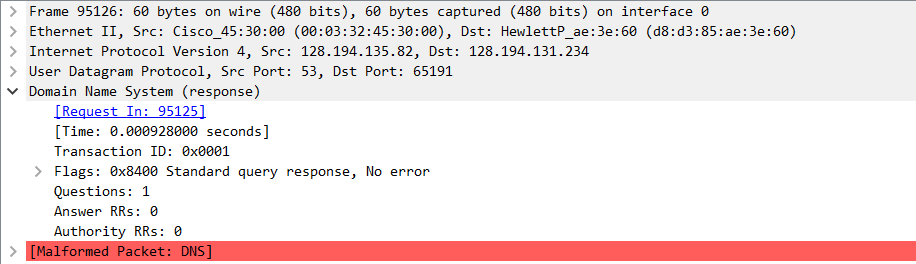
\includegraphics[width=11cm, height=3cm]{random3.irlWireShark}
\end{center}

We see that the packet is a malformed DNS packet further proving that the response is incorrectly formatted. 

\subsection{random5.irl}

The trace for \emph{random5.irl} using \emph{128.194.135.82} as the DNS server is shown below.

\begin{center}
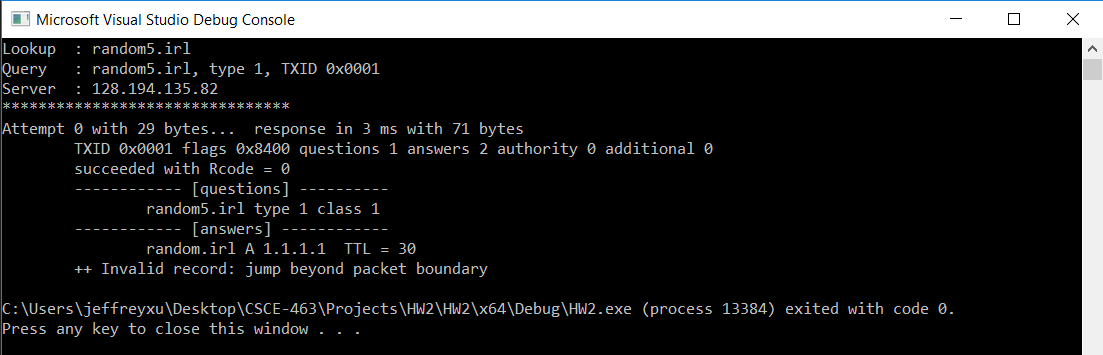
\includegraphics[width=11cm, height=3.8cm]{random5.irl}
\end{center}

We can see that on the second answer, there appears to be a jump that went beyond the packet boundary of 71 bytes. 

\subsection{random6.irl}

The trace for \emph{random6.irl} using \emph{128.194.135.82} as the DNS server is shown below.

\begin{center}
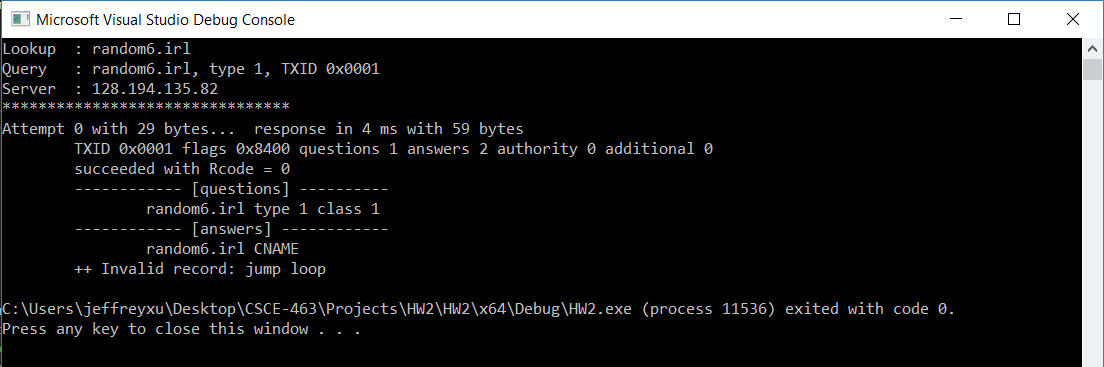
\includegraphics[width=11cm, height=3.8cm]{random6.irl}
\end{center}

We see that a jump loop seems to be present within the first answer. This is corroborated with the hex dump from Wireshark. 

\begin{center}
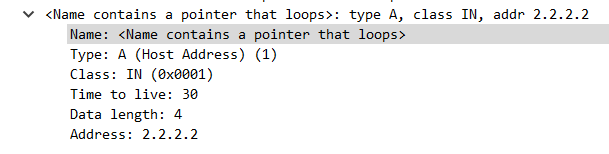
\includegraphics[width=11cm, height=3cm]{random6.irlWireShark}
\end{center}

\section{Case 2}

Now we want to see what outputs result from \emph{random1.irl} using the same DNS server. The output from the program is shown below.

\begin{center}
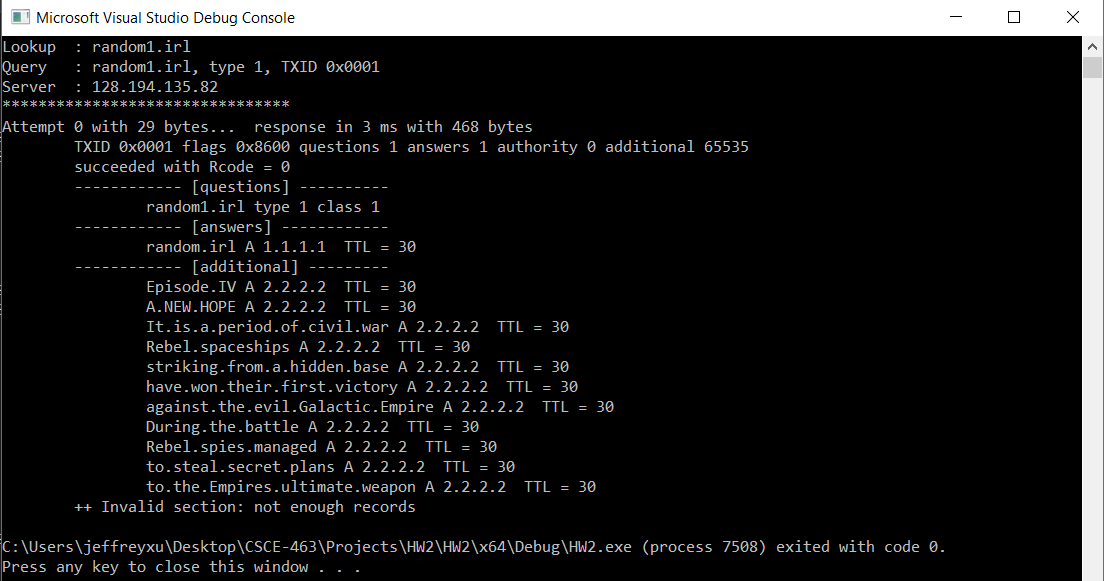
\includegraphics[width=11cm, height=5.2cm]{random1.irl}
\end{center}

We can clearly see that the \emph{additional} section does not contain enough records as there are 65536 additional records and the packet size doesn't even come close to containing that many records. 

\section{Case 3}

Now we need to check what \emph{random7.irl} gives us. The output from the program is shown below. 

\begin{center}
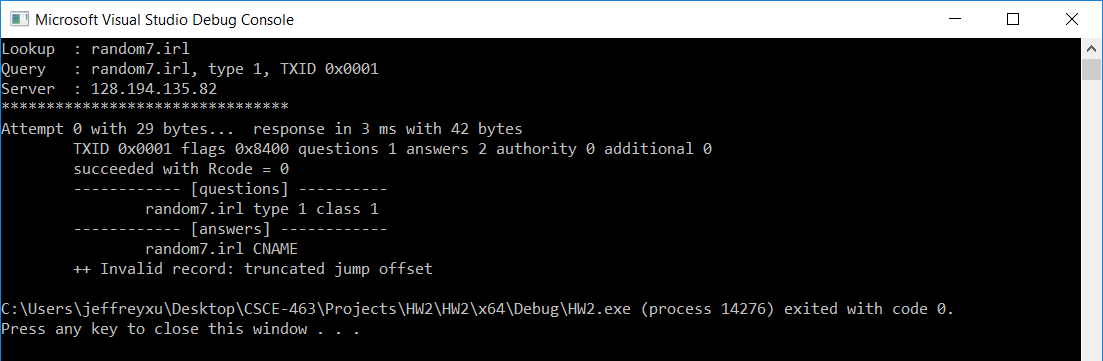
\includegraphics[width=11cm, height=3.9cm]{random7.irl}
\end{center}

We see that there appears to be a truncated jump offset which means that a jump was present but the packet ended before any offset information was provided. The Wireshark trace below shows more information. 

\begin{center}
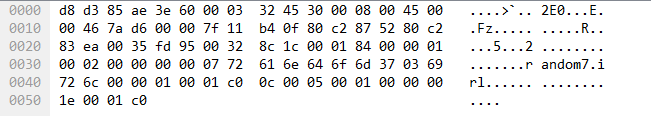
\includegraphics[width=11cm, height=2cm]{random7.irlWireShark}
\end{center}

We can see that the last byte of the packet is \emph{0XC0} but there's no jump information provided. 

\section{Case 4}

Now we want to test the different outputs that come from \emph{random4.irl}. Some of the outputs are shown below. 

\begin{center}
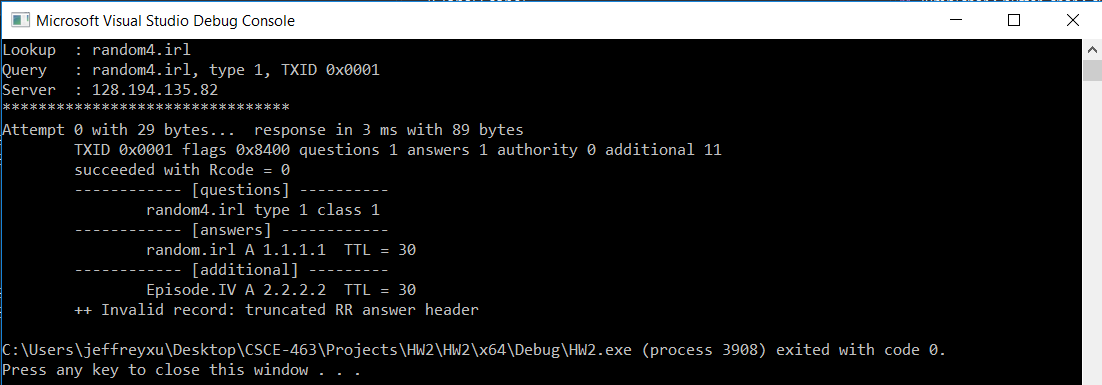
\includegraphics[width=11cm, height=4cm]{random4.irlTruncatedRR}
\end{center}
\begin{center}
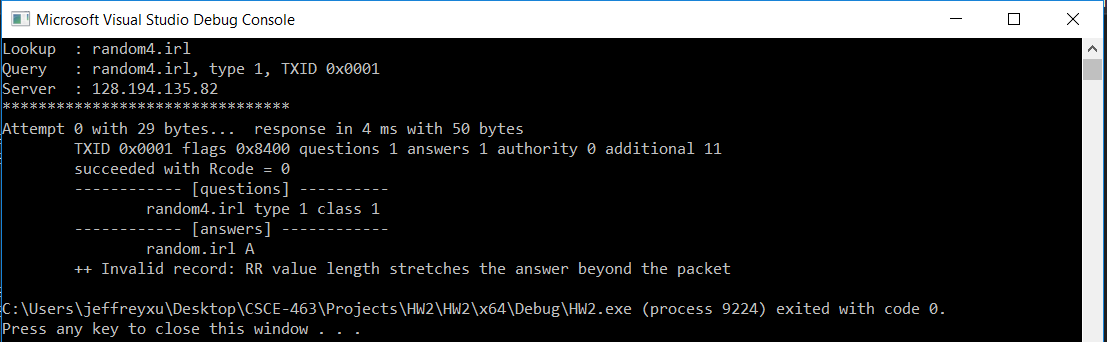
\includegraphics[width=11cm, height=3.8cm]{random4.irlRRLength}
\end{center}
\begin{center}
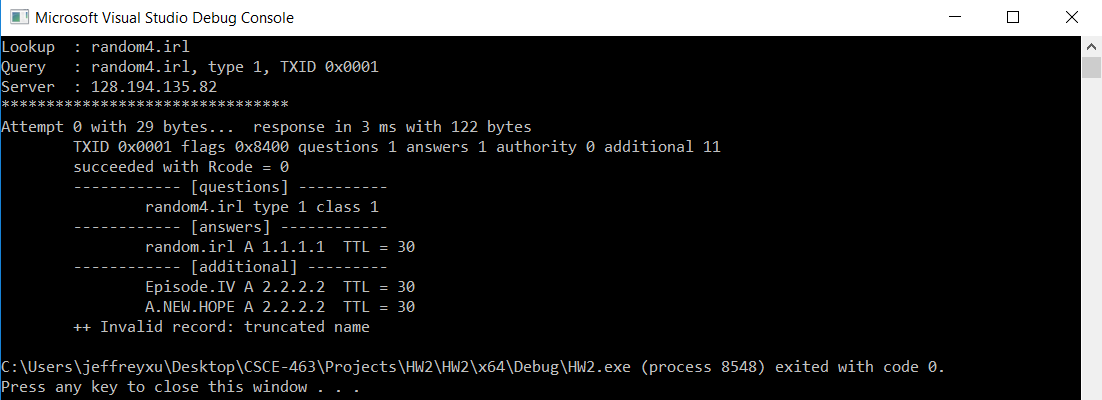
\includegraphics[width=11cm, height=4cm]{random4.irlTrancatedName}
\end{center}

We see that there is an output with a truncated RR answer header. To check for this case, I simply put an if-statement that checks if the current point plus the size of the RR answer header is greater than the total number of bytes. If so, then the program outputs the error message and quits the program. 

Another possible error message is that the RR value length stretches the answer beyond the packet. To check for this, I simply check if the length of the fixed RR header (length field of the RR header) goes beyond the packet, if so then we output the error and quit the program. 

Finally, we have the truncated name error message. To check for this error, I simply put another if-statement within the jump function that checks if the current block will go beyond the packet length. If so, then we output the error and quit the program. 

\section{Case 5}

Now we want to explore what \emph{random8.irl} is sending back and what algorithm is behind it that is creating the errors. From an initial testing of the host, it seems that the server is generating the same response packet each time, but truncating the packet at a random location within the packet. Some outputs from the host are shown below.

\begin{center}
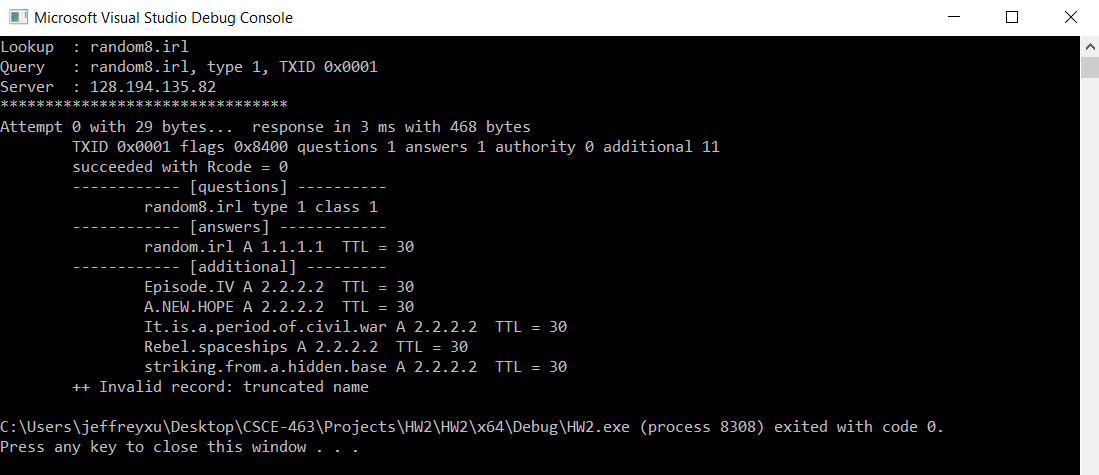
\includegraphics[width=11cm, height=4.5cm]{random8.irlCase1}
\end{center}
\begin{center}
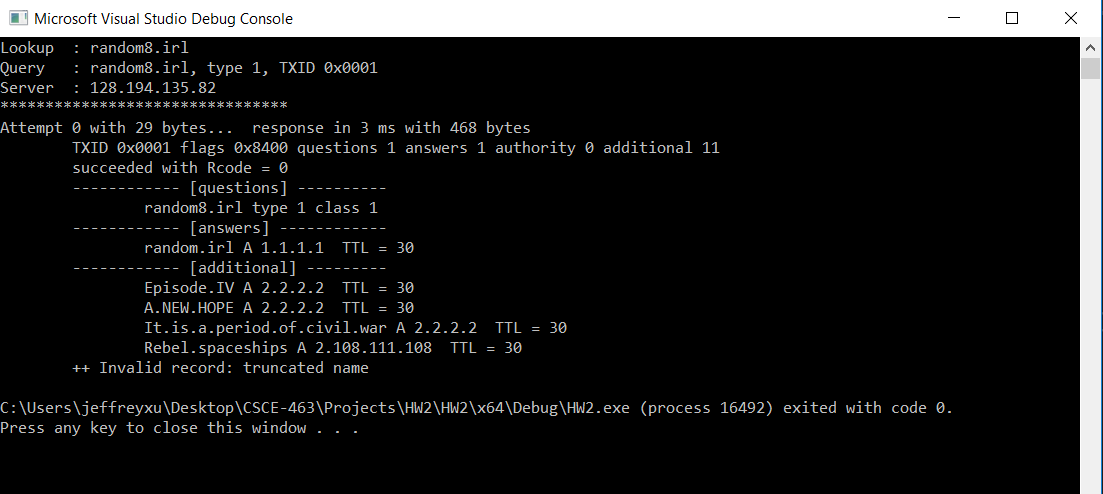
\includegraphics[width=11cm, height=4.4cm]{random8.irlCase2}
\end{center}
\begin{center}
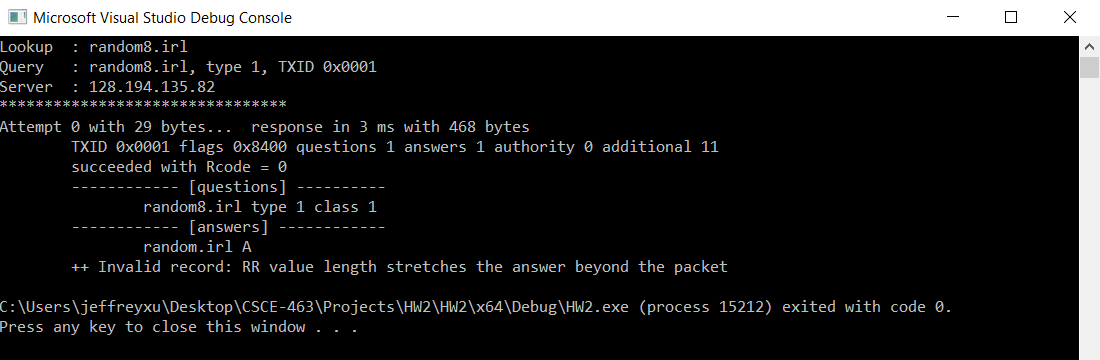
\includegraphics[width=11cm, height=3.8cm]{random8.irlCase3}
\end{center}

We see each time that there is always 1 question, 1 answer, and 11 additional records for the response. The order in which the response come are also in the same order with \emph{random.irl} as the answer, \emph{Episode.IV} as the first additional record, \emph{A.NEW.HOPE} as the next additional record and so on. As it occurs, the packet seems to be writing out the intro for Star Wars Episode IV but using the additional record names to output the words. 

I think that the server is probably putting illegitimate jumps and block sizes which would cause the issues of having truncated names, having the RR value go beyond the packet, having the issue of not having enough records (or what it seems based on the information in the packet), etc. 

If someone were to write a parser to parse these packets, they would most likely have to check all jump values and block size values when perform jumps to make sure that values are legit and don't cause an error. This only really needs to be done during the jump function since it seems that all issues occur when the program is jumping to read a name from another offset in the packet. 

\end{document}